\setchapterimage[7cm]{ztf_telescope.png} % Optionally specify the height
% \setchapterpreamble[u]{\margintoc}
\chapter{The Zwicky Transient Facility}
\labch{ZTF}
The second instrument relevant for this thesis is the Zwicky Transient Facility (ZTF). It is named after the notorious Swiss-American astronomer Fritz Zwicky, who e.g. first employed the Virial theorem to infer the existence of dark matter \sidecite{Zwicky1933}. Furthermore, together with Walter Baade, he posited the existence of supernovae and the creation of neutron stars in such events \sidecite{Baade1934}.

ZTF is a wide-field optical survey telescope. This means that it normally operates by scanning the full sky with a fixed cadence, in contrast to pointing to specific objects. It is located at Mount Palomar in California, United States, at 1700 m above sea level, roughly 130 km southeast of Los Angeles. Its optical system, the 1.2 m (48 inch) Samuel Oschin telescope, is a Schmidt design (see below) and was inaugurated in 1948 \cite{Harrington1952}. At the time of inauguration and for years to come, it was the largest Schmidt telescope in the world. Originally, the telescope used photographic plates, covering a field of view (FoV) of 44 square degrees. As these have obvious drawbacks, and because technological progress made it possible, the Near-Earth Asteroid Tracking (NEAT) program \sidecite{Pravdo1999} replaced the photographic plates with a charge-coupled device (CCD) camera in the early 2000s.\marginnote{See \url{https://sites.astro.caltech.edu/palomar/about/telescopes/oschin.html} for a historical overview.}

The camera was updated several times over the course of the next years. The immediate predecessor of ZTF, the Palomar Transient Factory (PTF) \sidecite{Law2009}, began operation in 2009. Equipped with a 96 Megapixel camera, it already had many of the characteristics of ZTF: A fully automated survey, searching for optical transients with a CCD camera.

PTF's successor in spirit, ZTF, contains the first electronic camera. With 47 square degrees, it covers almost the full FoV of the P48. The main design metric for ZTF was \textit{volumentric survey speed} \sidecite{Bellm2016}. This is the volume within which an object of given absolute magnitude can be detected in one exposure, divided by the total time for the exposure (observation plus overhead). The system saw first light in 2017, and started its scientific use in the year after. As of writing, it is still operational.

The two other telescopes located on Mount Palomar. The 1.5 m (60 inch) P60 telescope houses the SED Machine (SEDM) \sidecite{Blagorodnova2018}, a fully robotic, low-resolution spectrograph used for automatic classification of transients. The largest facility on the mountain is the 200-inch (5.1 m) Hale Telescope, which is used for optical and infrared photometry as well as mid- and high-resolution spectroscopy of fainter sources. Together, these telescopes form a natural hierarchy: ZTF is the discovery engine for optical transients. Promising sources are then classified with SEDM. If sources warrant it, deeper photometry and higher resolved spectroscopy can then be obtained with the big gun, the P200. All three telescopes are shown in Fig. \ref{fig:palomar_overview}.

\begin{figure*}[]
    \includegraphics{palomar_overview}
    \caption[View of Mt. Palomar]{View of Mt. Palomar with the three telescopes highlighted in the text. Image credit: Caltech, annotations added by the author.}
    \labfig{palomar_overview}
\end{figure*}

\section{Telescope Design}
A \textit{Schmidt telescope} is by design dedicated to taking images, contrary to earlier designs allowing actually looking through an eyepiece \sidecite{Schmidt1938}. For this reason, it is also referred to as a \textit{Schmidt camera}. The design goal is a wide FoV. This makes it the ideal instrument for sky surveys, where a large FoV maximizes the on-sky area that can be monitored. A Schmidt telescope combines a spherical mirror at the end of the telescope tube with an aspherical correcting lens (Schmidt plate) at the tube's entrance. The use of a spherical mirror combined with the correcting lens gets entirely rid of comatic aberration. Until the end of the 20th century, around ten Schmidt telescopes have been built, most of them to conduct sky surveys \sidecite{Cannon1995}. At least two of them were space telescopes: ESA's astrometry mission \textit{HIPPARCOS} \sidecite{ESA1997} (1989--1993) and the NASA explanet mission \textit{Kepler} \sidecite{Koch2010} (2009--2018). In both cases, the mission entailed monitoring of large areas of the sky; prime territory for Schmidt telescopes.

\begin{figure}[]
    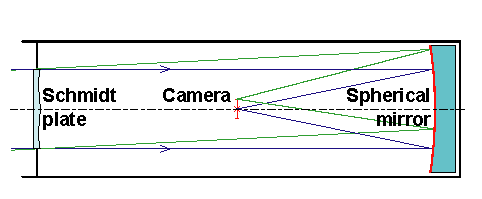
\includegraphics[width=1\textwidth]{schmidt_telescope_design.pdf}
    \caption[Schmidt telescope schematics]{Schmidt telescope schematics. Figure from \url{https://commons.wikimedia.org/wiki/File:Schmidt-Teleskop.svg}, annotations by the author.}
    \labfig{schmidt_telescope}
\end{figure}

\section{Camera}
The ZTF camera is a CCD design, consisting of 16 individual CCDs by commercial manufacturer e2v (\textit{Science CCD231-C6}), each having 6144x6160 pixels, resulting in a total camera resolution of $\approx 600$ Megapixels \sidecite{Dekany2016}. As one can see in Fig. \ref{fig:ztf_camera}, the array of 16 CCDs is slightly bent. This is necessitated by the Schmidt design, where the camera needs to be spherical, matching the spherical mirror. As individual CCDs are flat, each of the 16 sensors is is installed slightly tilted, tracing the overall curvature. To get rid of residual deviations from the global curvature, in front of each sensor a field flattener lens is mounted \sidecite{Bellm2019}.

CCDs are silicon-based light sensors. They consist of arrays of coupled metal-oxide semiconductor (MOS) capacitors, each one able to store the charge created by incident photons; one capacitor per pixel of the sensor array. The array is exposed to light for an amount of time (exposure time). During the exposure, incident photons create a charge proportional to the amount of light hitting each capacitor via the photo-electric effect. This charge is accumulated in each capacitor until the exposure is finished. To read out the CCD, the charges need to be moved to neighboring capacitors. When the MOS capacitors are tightly placed, one can move the charges from one capacitor to the next by changing the voltages on the capacitor's gates.

\begin{marginfigure}
    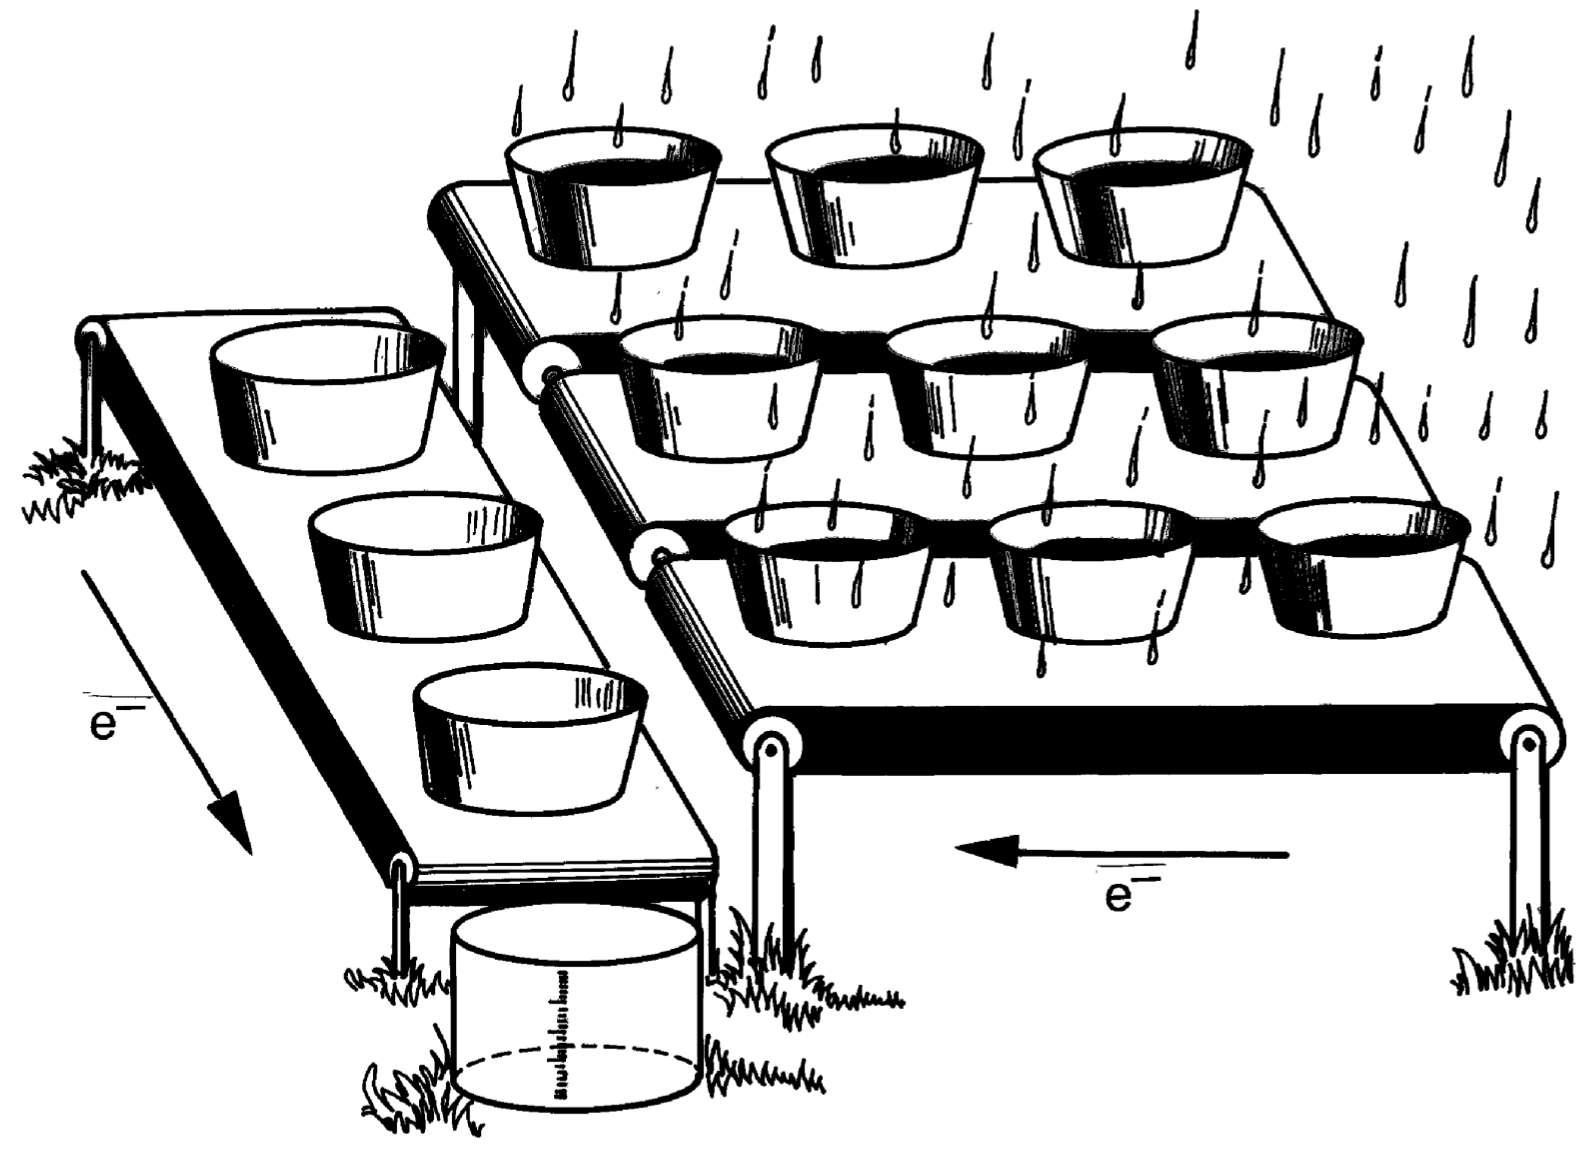
\includegraphics{ccd_buckets.png}
    \caption[CCD operational principle]{CCD operational principle, explained with buckets and rain water. From \cite{Janesick1987}.}
    \labfig{ccd_buckets}
\end{marginfigure}

In Fig. \ref{fig:ccd_buckets} the principle of a CCD is explained with little buckets collecting rain water. Each bucket symbolizes one capacitor or one pixel of the sensor array respectively. After the rain has stopped (the exposure is finished), each bucket naturally contains an amount of water proportional to the amount of water that rained down over it. Now the amount of water in each bucket (the charge deposited by incident light in each capacitor) needs to be measure. To do this, the buckets in each row are moved one position to the left with horicontal conveyor belts. Each bucket at the left end of the horicontal conveyor belt is then emptied into the bucket on the single vertical conveyor belt. The buckets of this vertical belt are then one by one drained into the meausuring bucket on the bottom left. After all buckets on the vertical belt are emptied, the process starts anew, until all buckets are empty. As one can see, the time this process takes scales linearly with the amount of buckets (or pixels) \sidecite{Janesick1987}. To speed up the process, one can subdivide the sensor area into smaller sections, which are read out in parallel.



The typical exposure for the ZTF camera is 30 seconds, while the readout time (emptying and measuring the charges in each capacitor) takes 8.2 seconds. Readout and digitization is done in parallel for four quadrants, each containing 4 CCDs. The four readout devices for the quadrants are \textit{Archon} CCD controllers by Semiconductor Technology Associates (STA). Each of these operates 16 simultaneous readout channels, four for each CCD. In summary, the camera is read out simultaneously in 64 independent regions to speed up the process.

An additional four smaller CCDs (2k x 2k pixels) are used as guidance, tip, tilt and focus sensors, with one additional Archon controller to read out these sensors \sidecite{Dekany2020}. To lower the thermal noise of the camera, it is placed on top of a cryostat cooling the CCDs to 160 K \cite{Dekany2016}.

\begin{figure}[]
    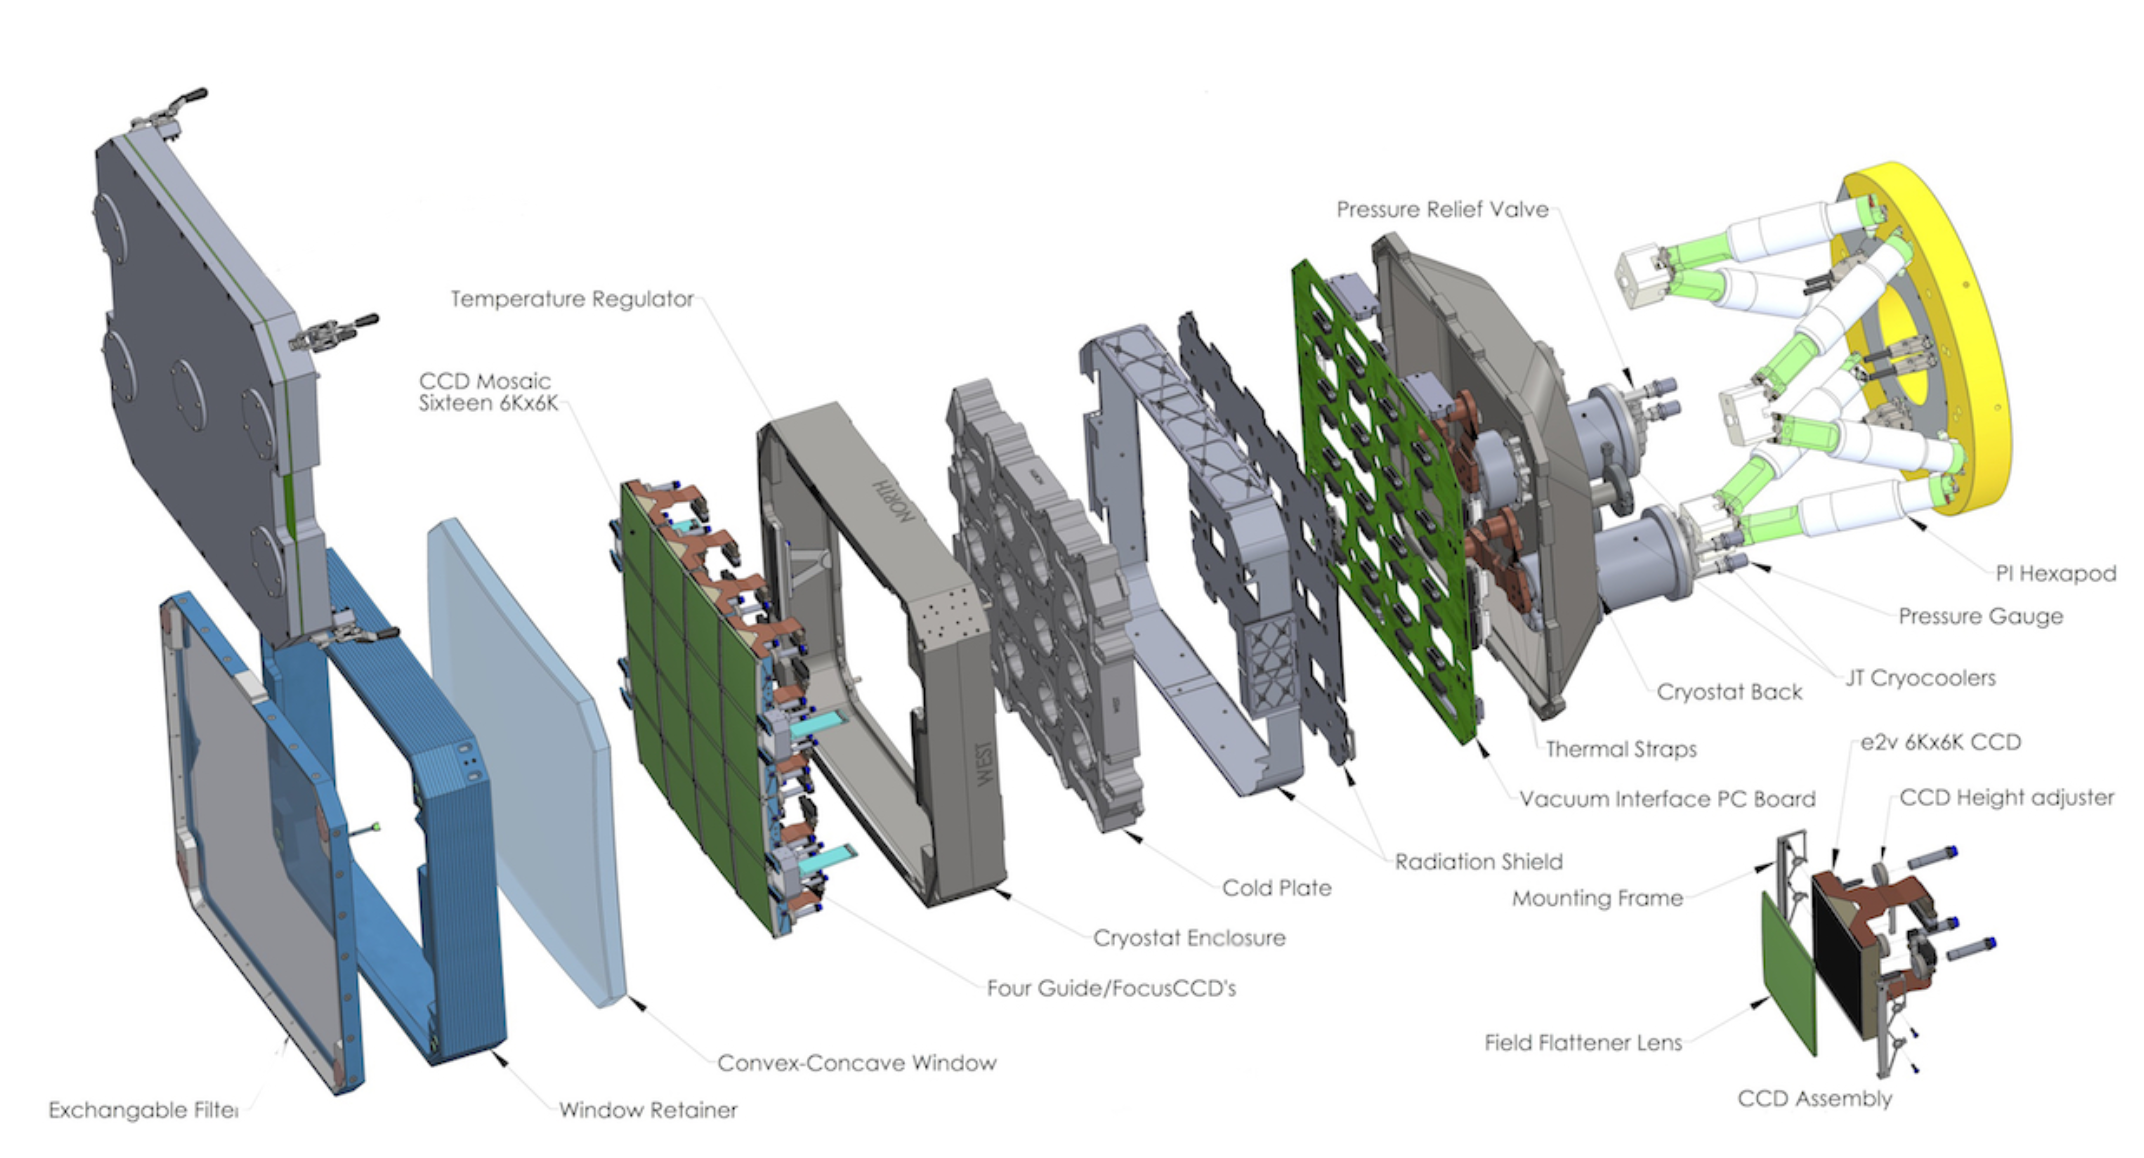
\includegraphics[width=1\textwidth]{ztf_camera.png}
    \caption[The ZTF Camera]{The ZTF camera. One can see the CCDs sandwiched between the filter on the front and the cryostat on the back. From \cite{Bellm2019}.}
    \labfig{ztf_camera}
\end{figure}

\section{Optical System}
\begin{marginfigure}
    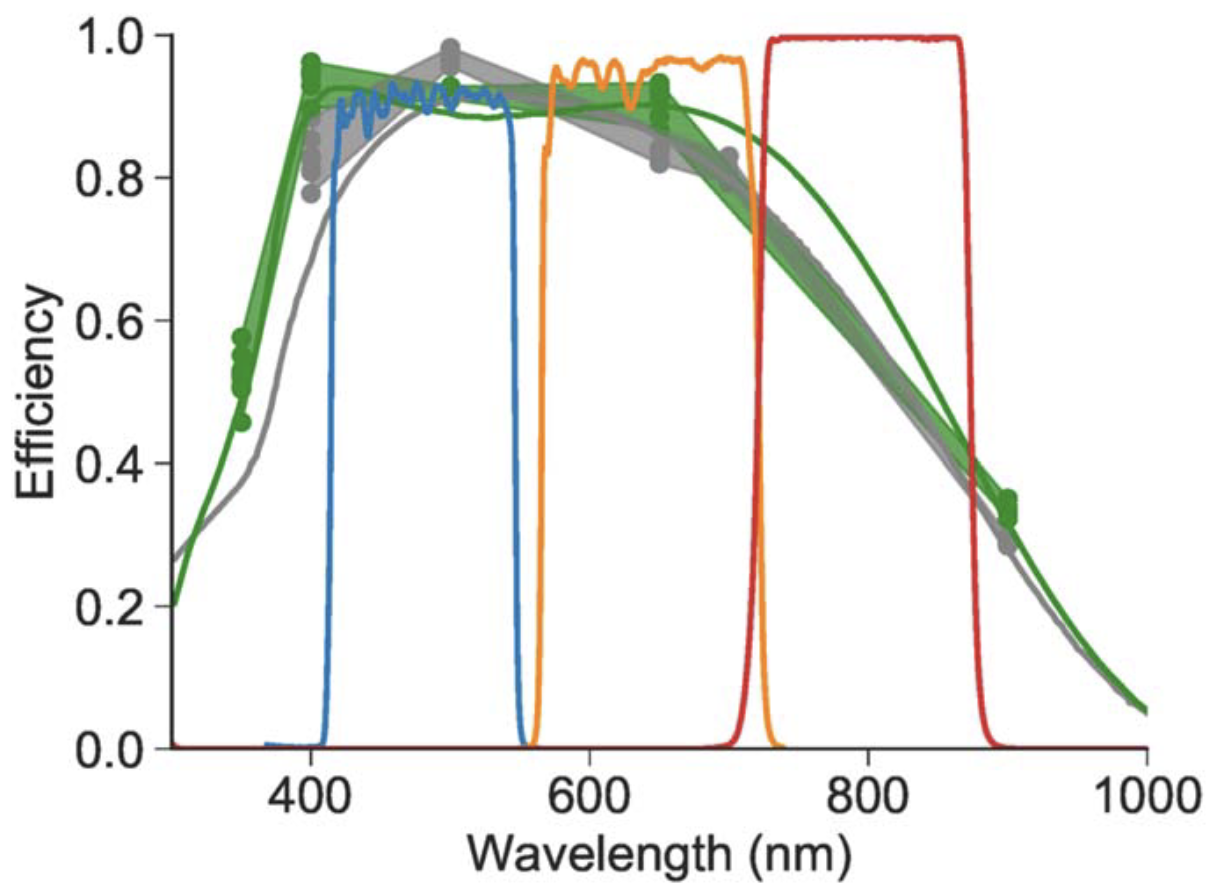
\includegraphics{ztf_throughput.png}
    \caption[ZTF Filter Transmission]{ZTF filter transmission for the three different bands (\textit{g}-band: blue, \textit{r}-band: orange, \textit{i}-band: red). The green and gray datapoints show the CCD quantum efficiency measurements (single and double-layer reflective coating). From \cite{Bellm2019}.}
    \labfig{ztf_transmission}
\end{marginfigure}

As the CCDs of the camera cannot ``see'' color, different filters need to be put in front of the camera to obtain color information. With ZTF, there are three different filters available: A \textit{g}-band filter with a median wavelength of 472 nm (corresponding to blue light), an \textit{r}-band filter (median wavelength: 634 nm, red light) and an \textit{i}-band filter (789 nm, near-infrared). These filters can be changed with a robotic arm, securely stowing the replaced filter and magnetically attaching the new one \cite{Dekany2020}.

The transmission of each filter and the CCD quantum efficiency curve can be seen in Fig. \ref{fig:ztf_transmission}. As one can see, the quantum efficiency starts to decrease within the \textit{r}-band towards higher wavelengths, rendering the \textit{i}-abnd the least sensitive ZTF band. The $5-\sigma$ median sensitivity for a 30s exposure reflects that fact. It is 21.1 mag in the \textit{g}-band, 20.9 in the \textit{r}-band and 20.2 mag in the \textit{i}-band for optimal conditions (new moon) \cite{Bellm2019}.

The main decision goal for the filter selection was to the maximize signal-to-noise ratio by avoiding major sky emission lines at Mt. Palomar while avoiding excessive costs. Not exactly matching the filters of potential calibrators (e.g. the Sloan Digital Sky Survey [SDSS]\sidecite{York2000}, PanSTARRS [PS1] \sidecite{Kaiser2002} or \textit{Gaia} \sidecite{Prusti2016}) was argued with the overall different telescope design of ZTF \cite{Bellm2019}.



\section{Image Processing}